\chapter{Authenticated Protocol pt. 1}

\begin{flushleft}
    I moderni sistemi informativi devono implementare dei controlli per l'\textbf{identificazione}, l'\textbf{autenticazione} e \textbf{autorizzazione} per gli utenti:
    \begin{itemize}[nosep]
        \item \textbf{identificazione}: bisogna garantire univocità nel riconoscimento di un utente.
        \item \textbf{autenticazione}: permette di prevenire che un'attaccante impersonifichi un attore legico.
        \item \textbf{autorizzazione}: determina a quali risorse un utente autenticato può accedere.
    \end{itemize}

    \textcolor{red}{\textbf{\textit{AutN} - Autenticazione}}: è il processo per determinare se un utente ha o meno \textbf{accesso} al \textbf{sistema}.
    
    \smallskip

    \textcolor{red}{\textbf{\textit{AutZ} - Autorizzazione}}: è il processo per regolare a quali risorse un utente autenticato è autorizzato ad accedere - la tipologia di regole che vengono applicate dipendono dal \textit{access model control} adottato.
\end{flushleft}

\begin{boxA}
    \textcolor{orange}{\textbf{Esempio - \textit{Authentication in WebApp}}}

    \begin{center}
        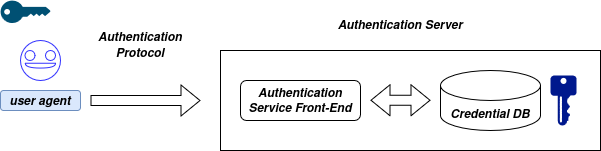
\includegraphics[width=0.75\textwidth]{img/web_app_auth.png}
    \end{center}

    È possibile estendere la complessità dell'architettura in modo da permettere \textbf{\textit{Single Sign On (SSO)}}, \textbf{\textit{Identity Federation (OpenID)}}, \textbf{\textit{Authorization delegation (OAuth2)}}, ma tutti questi hanno come blocco base (primitiva) l'autenticazione dell'utente.
\end{boxA}

\begin{flushleft}
    La procedura di \textbf{autenticazione} si basa su \textbf{fattori di autenticazione} (\textbf{\textit{authentication factor}}), ovvero dei metodi che utilizza un utente per dimostrare la sua identità, vengono anche chiamate \textbf{credenziali}. Ci sono diverse tipologie di fattori di autenticazione:
    \begin{itemize}[nosep]
        \item qualcosa \textbf{posseduto} dall'utente, ad esempio: \textbf{PIV - \textit{Personal Identifty Verification card}} o \textbf{U2F - \textit{Universal 2nd Factor}}.
        \item qualcosa \textbf{conosciuto} dall'utente, ad esempio una \textbf{password} o un \textbf{PIN}.
        \item Qualcosa che può essere eseguito dall'utente, tipologie di gesti.
    \end{itemize}
    Una procedura di autenticazione può richiedere ad un utente di fornire uno o più fattori di autenticazione - al giorno d'oggi è consigliato avere la \textbf{\textit{two-factor authentication}}.

    \medskip

    \textbf{Classi di Attacco}:
    \begin{enumerate}[nosep]
        \item attacchi \textit{client-side} (attacchi all'utente o al dispositivo dello stesso): possono essere ``\textbf{\textit{on-site}}'' ovvero un attacco allo \textbf{\textit{user-agent}} oppure attacchi ``\textbf{\textit{in motion}}'' quindi un attacco al canale di comunicazione, come ad esempio \textbf{\textit{snooping}}, \textbf{\textit{man-in-the-middle}} e \textbf{\textit{phishing}}
        \item attacchi \textit{server-side} che possono essere divise a loro volta in: \textbf{sfruttamento di \textit{weak credentials}} presenti nel servizio di autenticazione oppure \textbf{accesso alle credenziali del DB} anche noto come \textbf{\textit{data breach}}
    \end{enumerate}
\end{flushleft}

\section{Types of AuthN Protocol}

\begin{boxA}
    \textcolor{red}{\textbf{\textit{CAPTCHA - ``Turing Test''}}} \\
    Definiamo il concetto di utente: vogliamo differenziare gli ``umani'' da computer, anche detti \textbf{bot}. Vorremmo che l'autenticazione fosse riservata a persone, in modo da escludere bot che potrebbero essere degli \textit{exploit} eseguiti da un attaccante per automatizzare, ad esempio, il \textit{brute force} delle password. Il \textbf{CAPTCHA} è una procedura che ne ingloba altre, normalmente definite difficili o impossibili per un computer, per escludere che un utente sia un bot.

    \smallskip

    Un tipo particolare di CAPTCHA viene detto \textbf{reCAPTCHA} e si basa su degli input presi dal mondo reale. Spesso vengono fornite dalle aziende in maniera ``\textit{as-a-service}''
\end{boxA}

\begin{flushleft}
    \textcolor{red}{\textbf{\textit{Bearer Token}}} - \textit{basic authentication} \\
    Il protocollo di autenticazione più semplice è la dimostrazione di conoscere un segreto, che deve essere inviato al servizio ``\textit{as-is}'', ma deve essere ovviamente fatto attraverso un canale di comunicazione sicuro, nel caso opposto un avversario sarebbe capace di leggerlo. Il \textit{bearer token} può essere implementato in vari modi, ad esempio: password, \textit{API key}, \textbf{JWT}. Lo svantaggio maggiore è che se l'attaccante è capace di ottenere il segreto in transito è capace di \textbf{impersonificare permanentemente} l'utente - almeno finché la credenziale non verrà revocata.
\end{flushleft}

\begin{flushleft}
    \textcolor{red}{\textbf{\textit{One-time credentials}}} \\
    Permette di mitigare il danno in caso di accesso alla password sul canale di comunicazione tramite l'invio di \textbf{diverse \textit{authentication information} per ogni autenticazione}. Dopo ogni autenticazione il server \textbf{invalida} la credenziale utilizzata. Il \textcolor{olive}{\textbf{vantaggio}} è che anche violando il canale trasmissivo il danno è limitato, lo \textcolor{red}{\textbf{svantaggio}} è che il \textit{client} e \textit{server} devono riservare dello spazio propozionale al numero di procedure di autenticazione.
    
    \smallskip

    \textbf{\textit{Backup OTP codes}}: credenziali monouso pregenerate da mantenere offline in maniera sicura.
\end{flushleft}

\begin{flushleft}
    \textcolor{red}{\textbf{\textit{Challenge-Response}}} \\
    I protocolli del tipo \textit{challenge-response} consentono agli utenti di calcolare un valore in relazione ad una \textit{challenge} utilizzando le proprie credenziali utente. Le credenziali non vengono mai inviate attraverso il canale trasmissivo, e la sfida è monodirezionale per evitare attacchi del tipo \textbf{\textit{reply}}. Le credenziali potrebero non essere note all'utente ma solamente controllate. Alcuni esempi possono essere \textit{challenge} basate sul \textbf{tempo} (preso nell'istante di tempo iniziale della comunicazione, con una certa \textbf{tolleranza}) - nei server web è sempre presente (\textbf{NTP}) a differenza degli apparati embedded.

    \smallskip

    I protocolli \textit{challenge-response} possono essere implementati sia con crittografia \textbf{simmetrica} che tramite crittografia \textbf{asimmetrica}. In un caso la chiave di autenticazione è uguale a quella di verifica, nell'altro divergono.
\end{flushleft}

\begin{flushleft}
    \textcolor{red}{\textbf{\textit{Credential Ddatabases}}}: i database richiesti per permettere protocolli di autenticazione possono includere diverse tipologie di informazioni in relazione al tipo di protocollo utilizzato.
    \begin{itemize}[nosep]
        \item \textbf{\textit{bearer token}} (o informazioni derivate)
        \item \textbf{\textit{public keys}} (crittografia asimmetrica)
        \item \textbf{\textit{secret keys}}
        \item altri \textbf{metadati} o materiale crittografico
    \end{itemize}
    Il \textbf{database delle credenziali} è normalmente \textbf{statico} - a differenza \textcolor{red}{\textbf{\textit{dynamic credential database}}} che permette di aumentare la \textbf{resilienza} delle credenziali salvate modificandolo - il che implica che non varia durante tutta la procedura di autenticazione.
\end{flushleft}

\newpage

\section{OTP, OATH OTP}

\begin{flushleft}
    Andiamo ad analizzare i protocolli \textcolor{red}{\textbf{\textit{Challenge-Response based on Symmetric Cryptography}}}. \textbf{\textit{One-Time Password}} - è riferito alla credenziali $\neq$ password - sono funzioni \textit{challenge} che si basano sugli \textbf{HMAC}, esistono due standard:
    \begin{enumerate}[nosep]
        \item \textbf{HOTP, RFC4226 - \textit{Hash-based Ont Time Password}} è basato su un \textbf{HMAC} $\rightarrow \; \text{HTOP}(k, c) = \text{Truncate}(\text{HMAC}(k, c))$ dove $k$ è una \textbf{chiave}, $c$ è un \textbf{\textit{counter}} e la funzione $\text{Truncate}$ dipende dal livello di sicurezza che volgiamo garantire. In questo caso il \textit{client} non mantiene alcuno stato (ad eccezione della chiave) - a differenza del \textit{server} il cui stato è il \textbf{\textit{counter}} - quando il client vuole accedere, il server gli invia il \textbf{counter} e il client si riesce ad autenticarsi, contemporaneamente il server incrementa il counter.

        \begin{figure}[h]
            \centering
            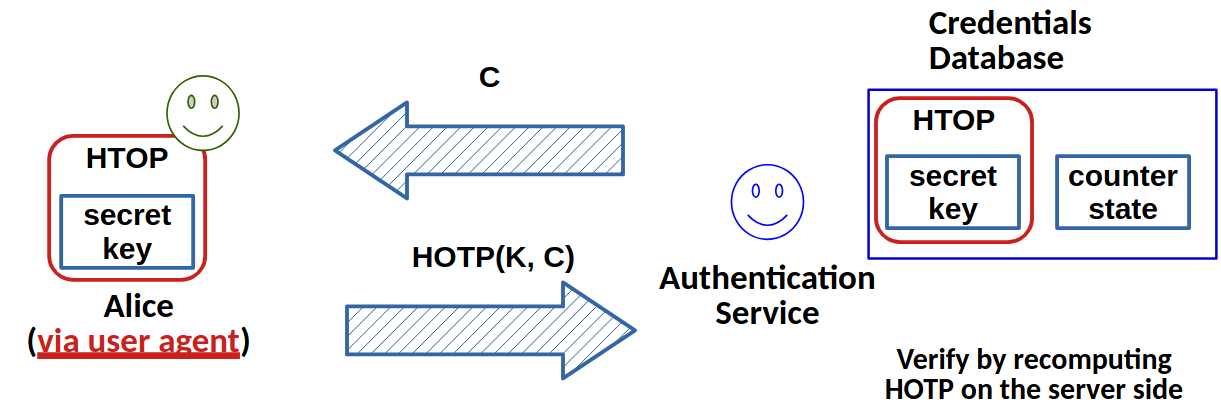
\includegraphics[width=0.65\textwidth]{img/hotp.png}
        \end{figure}

        Questo tipo di protocollo prova che Alice ha \textbf{controllo} sull'informazione secreta, ma potrebbe anche non averla - il segreto potrebbe essere gestito da un ``device'' differente tipo \textbf{\textit{Trust Platform Module - TPM}}. È possibile evitare di inviare esplicitamente la \textit{challenge} se abbiamo una sorgente comune (\textbf{variabile}) di informazioni, ad esempio il \textbf{tempo}.

        \begin{figure}[h]
            \centering
            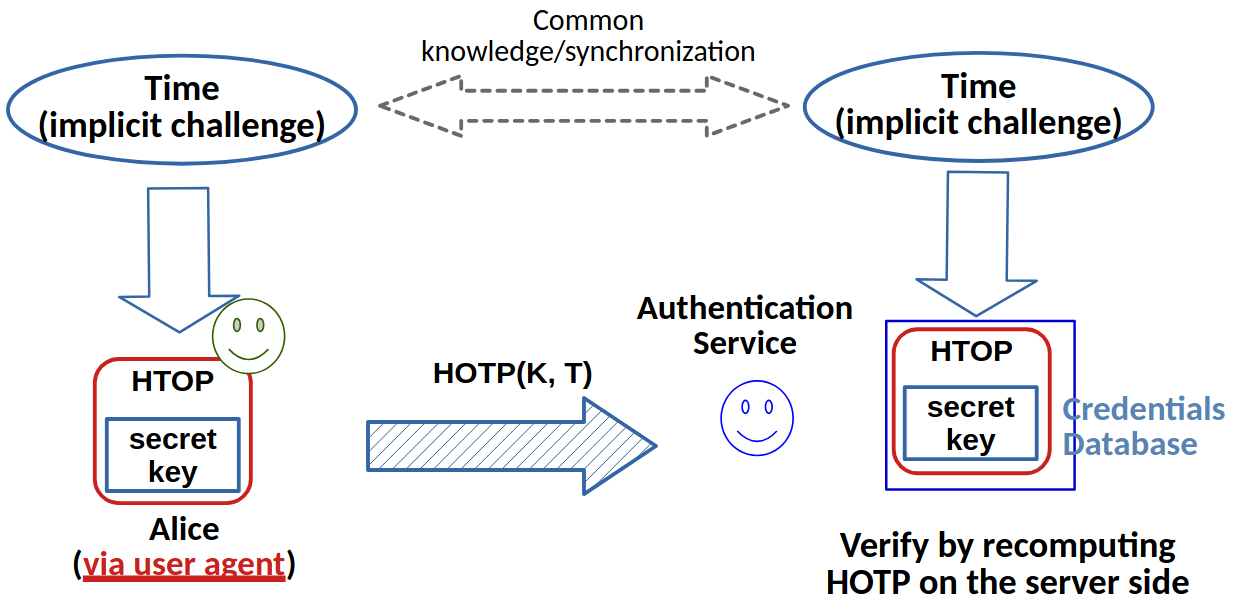
\includegraphics[width=0.65\textwidth]{img/hotp_1.png}
        \end{figure}

    \item \textbf{TOTP, RFC6238 - \textit{Time-Based One-Time Password}}: è un caso speciale dell'\textbf{HOTP}, infatti $\text{HTOP}(k, t) = \text{TOTP}(k, t)$ dove $t$ esprime \textbf{\textit{time step}} calcolati $t = \lfloor \frac{(\text{CurrentUnixTime} - T_0)}{X}$ dove $T_0$ è un tempo base Unix che decreta dove iniziare il conteggio, $X$ è il parametro che indica gli \textit{step} temporali. Assumiamo che client e server hanno accesso ad un'\textbf{informazione condivisa} - normalmente \textbf{\textit{UTC time}}.
    \end{enumerate}
\end{flushleft}

\section{Password e PIN}

\begin{flushleft}
    Il più semplice sistema di autenticazione richiesto ad un client è quello di fornire le sue credenziali, \textit{username:password}. L'utente invia le sue credenziali (attraverso un canale sicuro), il server esegue una \textit{query} al database per ottenere la password salvata per un certo username e poi effettua il confronto tra quella fornita e quella salvata.

    \smallskip

    \textbf{Definizione}: Le \textbf{password} sono dei segreti ricordabili dagli umani e quindi \textbf{deboli} per definizione. Questo non toglie la possibilità che utenti possano scegliere ``password forti'', ma nella maggior parte degli scenari dobbiamo assumere il contrario.

    \smallskip

    Andiamo a definere cosa vuol dire ``\textbf{segreto debole}'': un avversario può ``indovinare'' il segreto con un numero fattibile di tentativi. Il che può essere dovuto a:
    \begin{itemize}[nosep]
        \item \textbf{\textit{enumeration}}: con molti pochi tentativi, abbiamo un segreto ``molto debole'': \textbf{\textit{dictionary attack}}.
        \item \textbf{\textit{brute-forcing}}: il numero di tentativi diventa non trascurabile, numero limitato di password possibili.
    \end{itemize}

    \smallskip

    \textbf{Password}: segreti a bassa entropia, facilmente memorizzabili. Possono essere scelte corte e con un alfabeto ridotto. Anche password che non sono ``deboli'' possono diventare vulnerabili nel lungo periodo, infatti vengono considerate deboli in termini crittografici. \\
    \textbf{PIN}: segreti a bassa entropia (molto bassa), sono intrinsecamente vulnerabili a \textbf{ricerca esaustiva}, devono essere utilizzati solo in contesti vincolati dall'interfaccia per l'immissione.

    \medskip

    Un avversario può provare ad ``\textbf{indovinare}'' la password di un utente che sa che esiste, andando a fare richieste ripetute fino a che non riesce ad ottenere il login. 

    \begin{figure}[h]
        \centering
        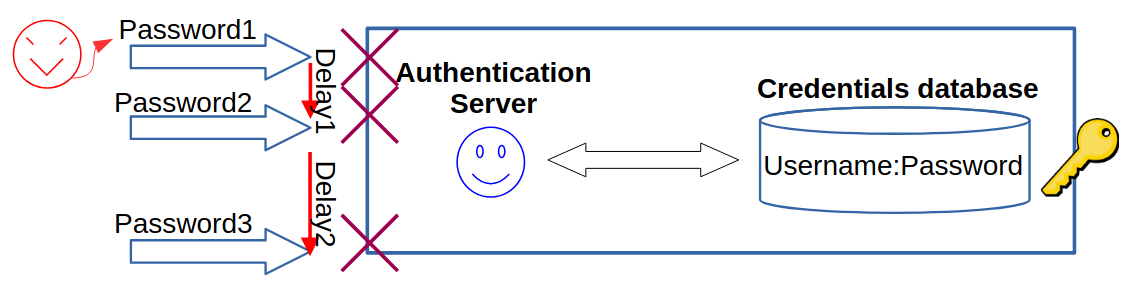
\includegraphics[width=0.55\textwidth]{img/int_attack.png}
        \caption{\textbf{\textit{Interactive Attack}}}
    \end{figure}

    Per conoscere il risultato del tentativo l'attaccante deve interagire con il server, per attenuare l'attacco il server può e deve applicare un \textbf{\textit{delay}} tra i tentativi del login per mitigare l'attacco di \textit{brute-force}. Con i \textbf{PIN} l'idea è la medesima, ma siccome sappiamo che il \textbf{PIN} è molto più debole è quindi necessario inserire un \textbf{numero massimo di tentativi} e in caso di mancata autenticazione si ricade in un altro sistema di \textbf{AuthN} più ``forte'' (\textbf{\textit{fallback}}). \\

    Libreria \textbf{python} per \textbf{HOTP} e \textbf{TOTP}: \textbf{\textit{pyotp}}.

\end{flushleft}

\section{Password Protection against Data Breaches}

\begin{flushleft}
    Focalizziamoci sul problema di \textbf{protezione delle password}, assumendo che il server sia completamente \textbf{compromesso} dall'avversario. I vincoli intrinsici che espone questa assunzione sono:
    \begin{enumerate}[nosep, start=0]
        \item non bisogna salvare le password in chiaro
        \item bisogna essere protettti conto \textit{pre-computational attacks}
        \item aumentare al protezione contro le password deboli.
        \item essere in grado di difenderci contro \textbf{attacchi ``specializzati''}
    \end{enumerate}

    \medskip

    \textcolor{red}{\textbf{[0] Non salvare le password in chiaro}}: salvare le password in chiaro comporta che se il server è completamente compromesso e l'attaccante ha accesso a tutte le coppie \textit{(username, password)}. La sua speranza è il riutilizzo della stessa coppia per altri applicazioni.

    \smallskip

    \textcolor{red}{\textbf{[1] Proteggere le credenziali nel database utilizzando le \textit{hash function}}}: in questo modo sarà possibile fare il confronto con il \textit{digest} salvato e il \textit{digest} ottenuto dall'applicazione della funzione hash alla password immessa dall'utente per autenticarsi. Siccome la funzione hash è \textbf{unidirezionale} se l'attaccante ha compromesso il sistema non sarà capace a partire dal \textit{digest} ottenere la password (\textbf{\textit{one-way}}).
    \begin{itemize}[nosep]
        \item se l'attaccante ottiene $H(p)$ dove $p$ è la password dell'utente, l'unico modo per ottenere $p$ è trovare una funzione inversa $H^{-1}$ (che dalle proprietà delle \textit{hash function} dovrebbe essere impossibile) oppure riuscire a trovare una password $p'$ (tramite \textbf{attacco esaustivo} sullo spazio delle password o con un \textbf{attacco a dizionario}) il cui \textit{digest} è uguale ad $H(p) = H(p')$
        \item quindi l'attaccante fallisce fintanto che $h$ è una funzione crittografica sicura? se le password venissero scelte come \textbf{chiavi crittografiche} allora \textbf{si}, nel caso in cui vengano scelte da un utente non paranoico allora \textbf{no}.
        \item infatti l'attaccate riesce a fare un \textbf{\textit{pre-computation attack}} potrebbe diminuire il tempo per trovare delle collisioni, soprattutto in caso di password corte; tipico esempio di \textbf{compromesso-spazio tempo} (possono essere violate anche password buone).
        \item non è possibile difendersi se l'avversario compromette la logica applicativa, quindi unicamente in caso di \textbf{\textit{data breach}}.
    \end{itemize}
\end{flushleft}
\begin{boxA}
    \textcolor{red}{\textbf{\textit{Pre-computation Attack to Credential Database}}}

    \begin{center}
        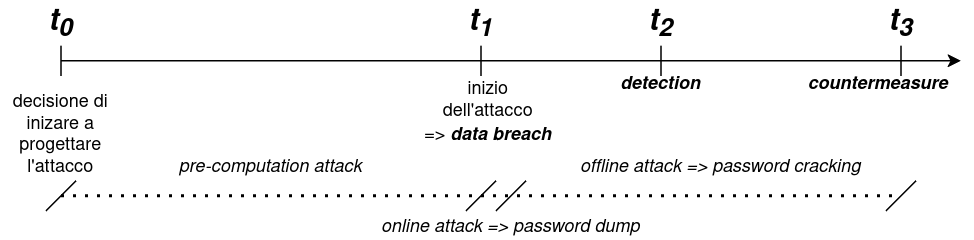
\includegraphics[width=\textwidth]{img/pre_attack_pwd.png}
    \end{center}

    L'obiettivo dell'attaccante è quello di ottenere una pre-immagine della password con l'hash non appena accede al database. Una possibilità sarebbe quella di \textbf{pre-calcolare} tutte le possibili password e il \textit{digest} corrispondente, la problematica di questa tipologia di approccio è che richiederebbe un mole memoria infattibile $\rightarrow$ \textbf{\textit{rainbow tables}} permettono di pre-calcolare attachi agli hash delle password senza dover memorizzare tutte le possibili corrispondenze per un dato \textit{domain}, la loro dimensione dimenta infattibile per lunghi input (16bytes alfanumerici).

    \smallskip

    $\Delta(t_0, t_1) \rightarrow 0$ in modo tale da limitare il tempo in cui un attaccante proverà l'\textit{offline cracking}, tramite il monitoraggio del traffico, del \textit{dark web} per osservare le \textit{disclosure} dei \textit{data breach} e segnalazione da parte di altri utenti.
\end{boxA}

\begin{flushleft}
    \textcolor{red}{\textbf{[2] Protezzione contro \textit{pre-computational attack} attraverso il \textit{Salt}}}: la difesa migliore è rendere \textbf{randomico l'\textit{hash function}}. Per ogni utente la password viene hashata con un differente valore \textbf{unico e randomizzato}, chiamato \textbf{\textit{salt}}, che viene salvato insieme al \textit{digest} nel database. Per ogni utente la sua riga di autenticazione sarà quindi formata da: 
    
    {\centering
        | \textit{username} | \textbf{\textit{salt}} | \textbf{\textit{hash(salt, password)}} |
    \par}

    In questo moto l'attaccante non può costruire la \textbf{\textit{rainbow table}} fino a che non ottiene il valore del \textbf{\textit{salt}}, ma siccome il valore del \textit{salt} viene ottenuto dall'attaccante durante la fase di \textbf{\textit{data breach}}, la generazione della \textit{rainbow table} avviene \textbf{online}, se si utilizzasse lo stesso \textit{salt} per più password una \textit{rainbow table} permetterebbe di aumentare l'efficenza del \textit{cracking} anche se online. In ogni caso l'attaccante è comunque capace di violare agilmente password deboli.

    \smallskip

    \textcolor{red}{\textbf{[2a] \textit{Secret Salt}}}, anche noto come \textbf{\textit{pepper}} è ottenibile dividendo l'\textbf{\textit{authentication server}} da un compomente esterno che genera il \textbf{\textit{secret salt}}, attraverso una \textbf{KDF}:

    {\centering
        \textbf{pepper} = \textbf{KDF}(\textbf{\textit{key}}, dimensione, ``\textbf{\textit{user}} || '\textbf{versione}')
    \par}
    
    Se viene compromesso questo componente esterno il \textit{fallback} è tornare all'utilizzo del \textbf{\textit{public salt}}, è anche importante ricordare che non è una soluzione semplice ed è difficilmente integrabile con framework di sviluppo web.

    \smallskip

    \textcolor{red}{\textbf{[3] Difendersi contro le password ``deboli''}}: introduciamo un nuovo \textbf{schema crittografico}: \textbf{\textit{password-based hash functions}}, chiamate \textcolor{red}{\textbf{\textit{PBKDF - Password-Based Key Derivation Functions}}}. Il loro obiettivo è quello di \textbf{aumentare} il tempo di esecuizione del calcolo dell'hash (\textit{slow down}) in modo tale che comunque rimanga \textbf{moderato}, ma che il suo inverso sia comunque \textbf{infattibile}. L'idea non è quella di bloccare completamente gli attacchi \textit{offline} delle password, se la password è debole è imposibile senza modificare anche l'architettura, ma cercare di \textbf{rallentarli} attacchi esaustivi \textbf{senza compromettere l'esecuzione del servizio legittimo}.
    \begin{itemize}[nosep]
        \item i ritardi devono essere valutati e aggiornati nel tempo in base all'hardware disponibile e al suo costo.
        \item se l'attaccante vuole andare più veloce, deve spendere di più.
    \end{itemize}

    Alcuni esempi di \textbf{PBKDF}:
    \begin{enumerate}[nosep]
        \item \textbf{PBKDF1}: procedura iterativa: $\underset{\text{n volte}, \; n \simeq 10^6}{\underbrace{H(H(...(H(}}\text{salt}, \text{password}))))$
        \item \textbf{PBKDF2}: in alcuni scenari potrebbe essere necessario utilizzare questa funzione perché approvata da molti standard.
        \item \textbf{Bcrypt}: supportata, comunemente, in scenari \textit{open-source}, anche questa ha un approccio iterativo.
    \end{enumerate}

    \smallskip

    \textcolor{red}{\textbf{[4] Difendersi contro attacchi ``specializzati''}}: gli attacchi specializzati utilizzano \textbf{hardware dedicato} per riuscire ad annullare (rendere trascurabile) il \textbf{gap} introdotto da funzioni ``lente''. Cercando, ad esempio, rendere le \textbf{PBKDF egalitarie} ovvero standardizzare nel tempo l'esecuzione indipendentemente dall'hardware sottostante.
    \begin{itemize}[nosep]
        \item negli anni '90 gli attaccanti avevano lo stesso hardware.
        \item negli anni '00 gli attaccanti utilizzavano le GPU.
        \item negli anni '10 gli attaccanti iniziano ad utilizzare hardware dedicati.
    \end{itemize}
    Il ritardo introdotto con le \textbf{PBKDF} è reso inutile visto il crescente gap di risorse (sia computazionali che economiche) tra gli attori legittmi e avversari.

    \smallskip

    Abbiamo detto che per mitigare queste tipologie di attacchi bisogna rendere le \textbf{PBKDF \textcolor{red}{egalitarie}}, idealmente, l'attaccante non deve essere capace di sfruttare il vantaggio che potrebbe dare architettura specializzate per ogni calcolo rispetto ad un attore legittimo.

    \smallskip

    \textcolor{red}{\textbf{memory-hard hash functions}}: siccome l'hardware dedicato normalmente vuol dire estremamente parallelizzato, ma normalmente queste disposibitivi (ad esempio GPU) hanno molta meno memoria rispetto ad una classica CPU. Pertanto se progettiamo un algoritmo che impieghi quanto più tempo se gli viene messa a disposizione quanta meno memoria evitiamo che gli aggressori possano forzarli in modo più efficiente rispetto agli attori legittmi. In sostanza \textbf{sono molto più lenti da calcolare se viene utilizzata poca memoria}.

    \begin{figure}[h]
        \centering
        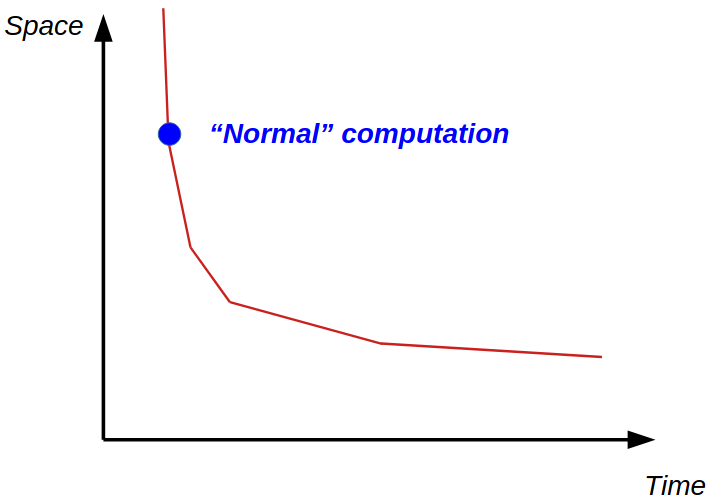
\includegraphics[width=0.35\textwidth]{img/mhf.png}
    \end{figure}

    Il primo algoritmo di questo tipo era \textbf{Scrypt} considerato sicuro, ma soffriva di due svantaggi: era vulnerabile ad una certa categoria di \textit{timing attacks} e il \textit{gap} tra attaccante e attore legittimo non era molto alto. \\
    Venne fatta una competizione per cercare un nuovo algoritmo (\textbf{\textit{password hasing competition}}) e nel 2015 il vincitore \textbf{Argon2} divenne lo standard per questo tipo di circostanze.
    \begin{itemize}[nosep]
        \item \textbf{Argon2i}: l'esecuzione è indipendente dal tempo rispetto agli input consigliata per l'utilizzo nei protocolli a chiave basati su password.
        \item \textbf{Argon2d}: è molto più forte, ma è dipendente dal tempo per quanto riguarda gli input, suggerito per l'uso di schema \textbf{PoW} o quando gli attacchi temporizzati non sono un problema.
        \item \textbf{Argon2id}: unisce le prime due \textit{mode of operation} (ibrido, spesso usato come default).
    \end{itemize}
    Parametri per \textbf{Argon2} :
    \begin{itemize}[nosep]
        \item \textbf{input}: la password inserita.
        \item \textbf{salt}: normalmente o 8 o 16 bytes.
        \item \textbf{\textit{time-cost}}: controlla il tempo di esecuzione (è simile al numero di replicazioni negli approcci iterativi); nel caso di esecuzioni per l'autenticazione \textit{online} siamo nel range 0.5-1.0 secondi, mentre per operazioni \textit{offline} anche più alto.
        item \textbf{\textit{memory}}: quantità di memoria richiesta per il calcolo ``normale'' (ad oggi il minimo per fine autenticativo 64MB, ma si può utilizzare anche 1GB per applicazioni critiche di sicurezza).
        \item \textbf{\textit{parallelism}}: numero di unità di calcolo parallele (anche se dipendenti).
        \item \textbf{\textit{output size}}: lunghezza del \textit{digest} (di default è 16 bytes).
    \end{itemize}
\end{flushleft}